\chapter{Signaux et systèmes discrets}
\section{Signaux discrets}
	\subsection{Signaux particuliers}
	Passant en revue certains signaux particuliers
	\begin{description}
	\item[Échelon unité]
	\begin{equation}
	\begin{array}{lll}
	u(n) &= 0 & n<0\\
	&=1 &n\geq 0
	\end{array}
	\end{equation}
	\item[Impulsion unité]
	\begin{equation}
	\begin{array}{lll}
	\delta(n) &= 0 & n\neq0\\
	&=1 & n=0
	\end{array}		
	\end{equation}
	\end{description}
	Ces deux signaux sont liés par les deux relations suivantes
	\begin{equation}
	\begin{array}{ll}
	u(n) &= \sum_{k=-\infty}^n \delta(k)\\
	\delta(n) &= u(n)-u(n-1)
	\end{array}
	\end{equation}
	\begin{description}
	\item[Exponentielle]
	\begin{equation}
	\begin{array}{ll}
	x(n) &= a^n\\
	x(n) &= e^{(\sigma+j\omega_0)n} = e^{\sigma n}(\cos\omega_0n+j\sin\omega_0n)
	\end{array}
	\end{equation}
	\item[Sinusoïdal]
	\begin{equation}
	x(n) = A\sin(\omega_0n+\Phi)
	\end{equation}
	\item[Périodique]
	\begin{equation}
	x(n) = x(n+N)\qquad \forall n
	\end{equation}
	\end{description}
	
	Intéressons nous à l'exponentielle complexe
	\begin{equation}
	x(n) = e^{j\omega_0n}
	\end{equation}
	On peut remarquer que si on considère $\omega_0' = \omega_0+2k\pi$, on retrouve 
	le même signal
	\begin{equation}
	e^{j(\omega_0+2k\pi)n} = e^{j\omega_0n}e^{j2k\pi n} = e^{j\omega_0n}
	\end{equation}
	Il est alors possible de restreindre la pulsation $\omega_0$ à $[0;2\pi[$. Cependant, 
	contrairement aux signaux continus, l'exponentielle complexe n'est pas toujours 
	périodique dans le cas discret.
	\begin{equation}
	\begin{array}{lll}
	&x(n)&=  x(n+N)\\
	\Leftrightarrow &e^{j\omega_0n} &= e^{j\omega_0(n+N)} = e^{j\omega_0n}e^{j\omega_0N}\\
	\Leftrightarrow &e^{j\omega_0N} &= 1\\
	\Leftrightarrow &\omega_0N &= 2m\pi \Longrightarrow \omega_0 = m\frac{2\pi}{N}
	\end{array}
	\end{equation}
	Il faut forcément que $\omega_0$ soit un multiple entier de $2\pi/N$. Or, nous avons 
	limité le domaine de $\omega_0$ : il n'existe que $N$ exponentielles distinctes de 
	période $N$ :
	\begin{equation}
	\Phi_k(n) = e^{jk\frac{2\pi}{N}n}\qquad k=0,1,\dots, N-1
	\end{equation}
	
	

		\subsubsection{Représentation d'un signal au moyen d'impulsions}
		\begin{wrapfigure}[8]{l}{7.5cm}
		\vspace{-5mm}
		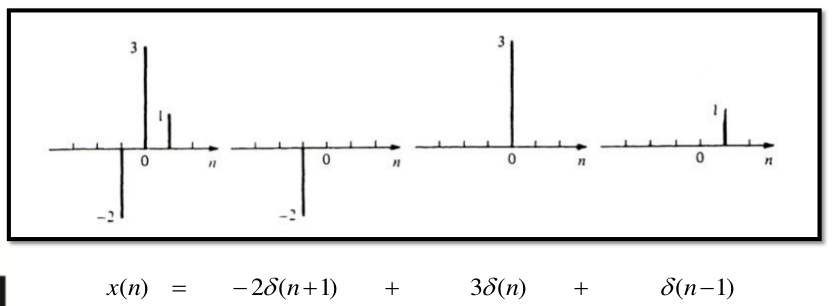
\includegraphics[scale=0.25]{ch2/image1.png}
		\captionof{figure}{ }
		\end{wrapfigure}
		Il est toujours possible d'écrire un signal $x(n)$ sous la forme
		\begin{equation}
		x(n) = \sum_{-\infty}^\infty x(k)\delta(n-k)
		\end{equation}\ \\
		\\
		
	
	
\section{Systèmes à temps discret, linéaires et permanents}
On appelle \textit{réponse impulsionnelle} $h(n)$ le signal de sortie lorsque le 
signal d'entrée est un delta de Dirac $\delta(n)$
\begin{equation}
h(n) = T[\delta(n)]
\end{equation}
Comme vu à la sous-section ci-dessus, écrivons un signal d'entrée sous la forme 
d'impulsion
\begin{equation}
x(n) = \sum_{-\infty}^\infty x(k)\delta(n-k)
\end{equation}
Les "bornes" de la somme sont telles que l'on sélectionne tout. La sortie devient 
\begin{equation}
y(n) = T\left[\sum_{-\infty}^\infty x(k)\delta(n-k) \right]
\end{equation}
Par linéarité, le système ne s'applique qu'à l'impulsion
\begin{equation}
y(n) = \sum_{-\infty}^\infty x(k)T\left[\delta(n-k) \right]
\end{equation}
Appliquons la propriété de permanence : rien ne change si on effectue cette opération 
à cet instant, ou plus tard :
\begin{equation}
y(n) = \sum_{-\infty}^\infty x(k) h(n-k)
\end{equation}
Il s'agit de la \textit{formule de convolution} (discrète) qui exprime la sortie en 
fonction de la réponse d'entrée pour tout signal
\begin{equation}
y(n) = x(n) * h(n)
\end{equation}
Le système est donc entièrement caractérisé par sa réponse impulsionnelle, $x(n)$ 
étant déjà connu. La convolution est commutative, on peut dès lors écrire
\begin{equation}
y(n) = h(n)*x(n) = \sum_{k=-\infty}^\infty h(k)x(n-k)
\end{equation}
	
	\subsection{Association de systèmes}		
		\subsubsection{Cascade}
		\begin{center}
		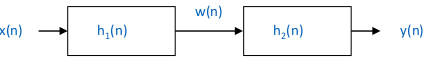
\includegraphics[scale=0.45]{ch2/image2.png}
		\captionof{figure}{ }
		\end{center}
		\begin{equation}
		\begin{array}{ll}
		w(n) &= x(n)*h_1(n)\\
		y(n) &= w(n)*h_2(n) = [x(n)*h_1(n)]*h_2(n)
		\end{array}
		\end{equation}
		
		\subsubsection{Convolution associative}
		\begin{center}
		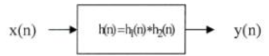
\includegraphics[scale=0.45]{ch2/image3.png}
		\captionof{figure}{ }
		\end{center}
		\begin{equation}
		y(n) = x(n)*[h_1(n)*h_2(n)] = x(n)*h(n)
		\end{equation}
	
		\subsubsection{En parallèle}
		\begin{center}
		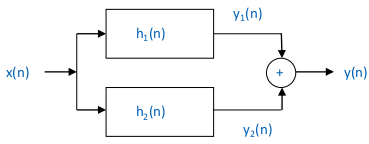
\includegraphics[scale=0.45]{ch2/image4.png}
		\captionof{figure}{ }
		\end{center}
		\begin{equation}
		\begin{array}{ll}
		y_1(n) &= x(n)*h_1(n)\\
		y_2(n) &= x(n)*h_2(n)\\
		y_n(n) &= y_1(n)+y_2(n) = x(n)*h_1(n)+x(n)*h_2(n)
		\end{array}
		\end{equation}
		
		\subsubsection{Distributive pour l'addition}
		\begin{center}
		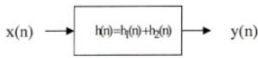
\includegraphics[scale=0.45]{ch2/image5.png}
		\captionof{figure}{ }
		\end{center}		
		\begin{equation}
		y(n) = x(n)*[h_1(n)+h_2(n)] = x(n)*h(n)
		\end{equation}
		
	\subsection{Stabilité}
	Nous avions précédemment vu la définition de la stabilité. La \textit{CNS} de stabilité 
	pour un SLP est
	\begin{equation}
	\sum_{k=-\infty}^\infty |h(k)|<\infty
	\end{equation}
\newpage
	\begin{proof}\ \\
	$\triangleright$ La condition est suffisante.\\
	Hypothèses :
	\begin{enumerate}
	\item $\sum_{k=-\infty}^\infty |h(k)|<\infty$
	\item Le signal d'entrée $x(n)$ est borné : $|x(n)| < A\quad \forall n$
	\end{enumerate}	 
	Calculons le signal de sortie
	\begin{equation}
	y(n) = \sum_{k=-\infty}^\infty h(k)x(n-k)
	\end{equation}
	Majorons
	\begin{equation}
	y(n) \leq \sum_{k=-\infty}^\infty |h(k)||x(n-k)|\leq A\sum_{k=-\infty}^\infty|h(k)|<\infty
	\end{equation}
	Le signal de sortie est borné, le système est donc stable.\\
	
	$\triangleright$ La condition est nécessaire.\\
	Nous pouvons choisir n'importe quel signal d'entrée, considérons ce signal particulier :
	\begin{equation}
	\begin{array}{lll}
	x(n) &= 1 &\text{ si } h(-n) \geq 0\\
	&= -1 &\text{ si } h(-n) < 0\\
	& \\
	x(n) &= \text{sign }h(-n)
	\end{array}
	\end{equation}
	Ce signal d'entrée est construit tel que le produit entre $h(n)*x(n)$ donne la valeur 
	absolue de $h$ : si $h$ est positif il ne se passe rien, si le signe est négatif le 
	signal multiplie par (-1) de sorte à avoir un signe positif. Ce signal est bien borné
	\begin{equation}
	|x(n)| = 1
	\end{equation}
	Calculons l'échantillon de sortie $y(0)$ :
	\begin{equation}
	y(0) = \sum_{k=-\infty}^\infty h(k)x(-k) = \sum_{k=-\infty}^\infty |h(k)|
	\end{equation}
	La sortie $y(0)$ ne sera borné que si la réponse impulsionnelle est absolument sommable, 
	la condition est bien nécessaire.	
	\end{proof}		
	
	\subsection{Causalité}
	Par définition $y(n)$ n'est causal que s'il dépend de $x(n)$ mais pas de $x(n+1),\dots$. 
	Pour que $y(n)$ ne dépende pas de $x(k)$ pour $k>n$, il faut que $h(n)=0$ pour $n<0$, 
	soit la CNS de causalité. La réponse impulsionnelle doit être causale, il faut alors 
	stopper la somme à $n$
	\begin{equation}
	y(n) = \sum_{k=-\infty}^n x(k)h(n-k) = \sum_{k=0}^\infty h(k)x(n-k)
	\end{equation}
	
\section{Systèmes décrits par une récurrence linéaire}
La récurrence linéaire est définie par
\begin{equation}
\sum_{k=0}^N a_ky(n-k) = \sum_{k=0}^M b_kx(n-k)
\end{equation}
Il en résultera une $ED$ donnant lieu à une infinité de solution : on impose des CI pour 
garantir l'existence et l'unicité de la solution (cf. \textit{Analyse I, II} et $III$).

\exemple{Considérons la récurrence du premier ordre
\begin{equation}
y(n) -ay(n-1) = x(n)\quad \Longrightarrow \quad y(n) = x(n) + ay(n-1)
\end{equation}
Considérons initialement une condition de repos et le signal d'entrée suivant :
\begin{equation}
x(n) = b\delta(n)
\end{equation}
On a alors
\begin{equation}
\begin{array}{lll}
y(-1) &= x(-1) &=0\\
y(0) &= x(0) + ay(-1) &= x(0) = b\\
y(1) &= x(1)+ay(0)&=ab\\
y(2) &= x(2)+ay(1) &= a^2b\\
y(n) &= x(n)+ay(n-1) &= a^nb
\end{array}
\end{equation}
La solution particulière vaut alors
\begin{equation}
y(n) = a^nbu(n)
\end{equation}

Vérifions que ceci est bien solution de $x(n) = y(n)-ay(n-1)$ avec
\begin{equation}
\left\{\begin{array}{ll}
y(n) &= a^nbu(n)\\
y(n-1) &= a^{n-1}bu(n-1)
\end{array}\right.
\end{equation}
Après substitution dans l'équation de récurrence, on trouve
\begin{equation}
a^nb(u(n) - u(n-1)) = b\delta(n)
\end{equation}
En effet, $(u(n) - u(n-1))$ n'est rien d'autre que l'impulsion. Cependant, nous 
avons un facteur $a^n$ en trop. Est-ce une erreur ? Discutions en fonction de $n$
\begin{equation}
a^nb\delta(n)=b\delta(n) \left\{\begin{array}{ll}
\text{Si }\ n=0 & a^0b\delta(0)=b\delta(0)=b\\
\text{Si }\ n\neq 0 & a^nb0=b0=0
\end{array}\right.
\end{equation}
Notre solution particulière est bien solution ! Il reste à calculer la solution 
générale de la récurrence homogène
\begin{equation}
y(n) -ay(n-1) = 0
\end{equation}
La solution sera $y(n)=ka^n$ (on peut vérifier que c'est bien le cas). En imposant
\footnote{Choix arbitraire donnant un résultat propre, mais ici non linéaire ! Pour 
avoir une solution linéaire, il aurait fallu poser $y(-1)=0$. L'avantage de considérer 
en $(-1)$ est que l'échelon $u$ s'annule.} $y(-1)=c$, 
on trouve comme S.\textbf{G}. (SGEH + SPEnH) :
\begin{equation}
y(n) = ca^{n+1}+ba^nu(n)
\end{equation}
La solution au système linéaire étant \textit{causal}, on dit ciao-ciao au terme en $n+1$ :
\begin{equation}
y(n) = a^nbu(n)
\end{equation}
Si le signal d'entrée est une impulsion de Dirac $\delta(n)$, le signal de sortie sera la 
réponse impulsionnelle. Posons $b=1$
\begin{equation}
h(n) = a^nu(n)
\end{equation}}

\newpage
\exemple{\ \\
Nous avons ainsi entièrement caractérisé notre SLP. Voyons ce que vaut le signal de sortie 
pour un échelon unitaire
\begin{equation}
\begin{array}{ll}
y(n) &= \sum_{k=-\infty}^\infty x(k)h(n-k)\\
&= \sum_{k=-\infty}^\infty u(k)a^{n-k}u(n-k)\\
&= \sum_{k=0}^\infty a^{n-k}u(n-k)\\
&= \sum_{k=0}^n a^k
\end{array}
\end{equation}
Il est possible de retrouver cette réponse en partant directement de la relation de 
récurrence, comme l’illustre le slide T22.
}















	
	
	
	
	
	
	
	
	
	
	
	
	
	
	
	
	